\documentclass{article}
\usepackage{microtype}
\usepackage{graphicx}
\usepackage{booktabs}
\usepackage{hyperref}
\usepackage{icml2026}
\usepackage{amsmath,amssymb,amsthm}
\usepackage{array}
\newtheorem{proposition}{Proposition}
\newtheorem{corollary}{Corollary}
\newcommand{\E}{\mathbb{E}}
\newcommand{\Prob}{\mathbb{P}}
\newcommand{\muh}{\widehat\mu}
\newcommand{\argmax}{\mathop{\rm arg\,max}}
\newcommand{\SynOptimism}{9.7}
\newcommand{\SynNaiveCover}{32.9}
\newcommand{\SynAuditCover}{96.8}
\newcommand{\SynSimultaneousCover}{97.9}
\newcommand{\SynNaiveFalseSuperiority}{43.8}
\newcommand{\SynAdjustedFalseSuperiority}{1.7}
\newcommand{\RealOptimism}{4.7}
\newcommand{\RealNaiveCover}{80.8}
\newcommand{\RealAuditCover}{96.5}
\newcommand{\RealSimultaneousCover}{98.4}
\newcommand{\RealReportedGain}{6.2}
\newcommand{\RealActualGain}{1.5}
\newcommand{\RealNaiveFalseSuperiority}{3.6}
\newcommand{\RealAdjustedFalseSuperiority}{0.2}
\newcommand{\RealAuditReferencedOptimism}{5.8}
\newcommand{\RealOptimismQFive}{0.6}
\newcommand{\RealOptimismQNinetyFive}{9.0}
\newcommand{\RealNegativeRate}{3.1}
\newcommand{\HeteroLargeOptimism}{2.3}
\newcommand{\HeteroLargeOptimal}{86.7}
\newcommand{\RealMeanReportedAccuracy}{19.9}
\newcommand{\RealWeightedAuditAccuracy}{14.2}
\newcommand{\RealAuditReferenceAuditSE}{0.58}
\newcommand{\RealAuditReferenceMCSE}{0.04}
\newcommand{\MatchedQualityDifference}{-0.03}
\newcommand{\MatchedQualitySE}{0.02}
\newcommand{\MatchedAuditWidth}{12.3}
\newcommand{\MatchedAuditCoverage}{96.3}
\newcommand{\MatchedSimWidth}{22.1}
\newcommand{\PrimaryTuneScore}{16.4}
\newcommand{\PrimaryBaselineTune}{10.2}
\newcommand{\PrimaryAuditScore}{15.5}
\newcommand{\PrimaryBaselineAudit}{14.0}
\newcommand{\PrimaryAuditGain}{1.6}
\newcommand{\PrimaryCandidate}{1}
\newcommand{\PrimaryLo}{13.4}
\newcommand{\PrimaryHi}{17.9}
\newcommand{\PrimaryGainLo}{-2.7}
\newcommand{\PrimaryGainHi}{5.9}
\newcommand{\PrimaryP}{0.148}
\newcommand{\PrimaryWins}{111}
\newcommand{\PrimaryLosses}{95}
\newcommand{\MeanCorrelation}{0.17}
\newcommand{\MinCorrelation}{-0.04}
\newcommand{\MaxCorrelation}{0.70}
\newcommand{\MinDev}{11.8}
\newcommand{\MaxDev}{17.4}
\newcommand{\TotalResponses}{49,152}
\newcommand{\EvaluatedTokens}{11,243,832}
\newcommand{\InferenceHours}{10.36}
\newcommand{\ComputedTokens}{8,377,636}
\newcommand{\MaxPrompt}{995}
\newcommand{\ServerCpuHours}{36.34}
\newcommand{\PeakMemoryGiB}{10.29}

\icmltitlerunning{Auditing Scores and Gains After Prompt Search}
\begin{document}
\twocolumn[
\icmltitle{What Survives Prompt Search?\\Auditing Scores, Gains, and Confidence After Benchmark Reuse}
\begin{icmlauthorlist}
\icmlauthor{Anonymous Author}{anon}
\end{icmlauthorlist}
\icmlaffiliation{anon}{Anonymous Institution}
\icmlcorrespondingauthor{Anonymous Author}{anonymous@example.invalid}
\icmlkeywords{language model evaluation, prompt optimization, post-selection inference}
\vskip 0.3in
]
\printAffiliationsAndNotice{}

\begin{abstract}
An automatically selected prompt is often evaluated on the questions that selected it, conflating configuration quality with favorable sampling noise. We study exhaustive search over a frozen finite family, distinguishing the accuracy of the selected configuration, the expected accuracy of the search procedure, and a gain over a fixed baseline. A dependence-sensitive analysis and controlled Bernoulli experiments show why the number of distinct candidates and their shared errors both matter: with equally accurate candidates, an ordinary nominal 95\% interval covers only \SynNaiveCover\% after a search over 64 independent candidates on 128 questions. We generate \TotalResponses\ real answers from Qwen2.5-0.5B-Instruct on MMLU-Pro, finding \RealOptimism\ percentage points of mean optimism for a 24-prompt, 128-question search in an empirical-population replay; a separate locked audit does not establish superiority over a fixed baseline. Exact simultaneous intervals protect a frozen family, while an independent audit protects any configuration chosen without its feedback. A comparison with exactly matched model-call budgets shows how to evaluate the winner separately while measuring the corresponding loss in selection quality; our guarantees and coverage experiments are explicitly limited to their respective sampling targets.
\end{abstract}

\section{Introduction}
Automatic prompt and program optimization makes benchmark evaluation a learning problem. A system searches instructions, demonstrations, or compositions of model calls, picks the highest scoring configuration, and subsequently uses that configuration. The score used to make this choice has two roles: it is an optimization objective and a proposed measurement of performance. Those roles need not agree, even when every individual answer is scored correctly and no benchmark answer is placed in a prompt.

Consider a search among configurations that actually have the same accuracy. On a finite question set, some obtain favorable errors and become winners. Their reported improvements are entirely sampling effects, but an ordinary confidence interval calculated after selection treats the winner as if it had been fixed in advance. Conversely, if the search genuinely discovers a better prompt, its reported improvement can contain both a real gain and selection noise. Establishing that a selected score is optimistic does not establish that optimization was useless.

This work asks what a reported number can support after a finite prompt search. Our unit of analysis is a vector of responses to the \emph{same question} across candidates, preserving the dependence that comes from shared item difficulty and shared model behavior. This matters because independent-arm models can greatly exaggerate the effective search size, while treating all prompts as one can conceal substantial selection noise. We study both point estimates and decisions: a falsely claimed improvement over a fixed baseline is a different failure from inaccurate absolute accuracy.

We contribute a reproducible audit with three linked parts. First, we separate the relevant estimands and give an elementary contrast-variance bound explaining how shared noise cancels. Second, we measure optimism, interval coverage, and false superiority under controlled dependence and in a matrix of newly generated real-model responses. Third, we compare conventional simultaneous inference with a locked audit under a precisely matched number of model calls, including the effect on the quality of the selected configuration. These are standard inference tools used in an explicit reporting protocol, rather than a new general solution to adaptive data analysis.

\section{Related Work and Scope}
\paragraph{Prompt optimization and sensitivity.}
DSPy represents language model programs as optimizable modules \citep{khattab2023dspy}; MIPRO jointly searches instructions and demonstrations for multistage programs \citep{opsahl2024mipro}. Budgeted prompt selection can be formulated as best arm identification \citep{shi2024efficient}. These works motivate the selection mechanism, but choosing a strong candidate and honestly measuring its accuracy are distinct objectives. We implement a transparent exhaustive search, not DSPy or MIPRO, and make no empirical claim about the reporting practices of those implementations.

Prompt formatting can substantially change model behavior \citep{sclar2024quantifying}. PromptEval estimates a performance distribution across many templates by borrowing information across prompts and examples \citep{polo2024efficient}. A distribution over prompt accuracies describes sensitivity; it is not itself a confidence interval for the configuration selected on noisy scores. MMLU-Pro provides challenging questions and studies prompt stability \citep{wang2024mmlu}. Our real experiment uses that dataset with a small constrained-decoding model and explicitly does not reproduce its standard chain-of-thought evaluations.

\paragraph{Inference after reuse.}
Adaptive data analysis studies validity when analyses are generated using previous data feedback \citep{dwork2015preserving}. The Ladder addresses a reusable competition leaderboard \citep{blum2015ladder}. Our fixed-family setting is narrower: simultaneous inference suffices without a reusable-holdout mechanism. Gaussian approximations and multiplier bootstrap methods can exploit dependence among many statistics \citep{chernozhukov2013gaussian}; we use an exact, conservative finite-family comparator instead of claiming small-sample bootstrap validity. The contribution here is the linked evaluation of scores, comparison decisions, and evaluation cost, not the observation that selection can bias reported results. To preserve independent investigation under the study constraints, literature access was restricted to the supplied sources and direct official infrastructure pages; this is not an exhaustive priority review.

\section{What Is Being Estimated?}
Let $Z\sim P$ be a question, including its gold answer, and index a frozen family of $K$ configurations by $j=0,\ldots,K-1$, with candidate 0 fixed as the baseline. A configuration includes the prompt, model, decoding procedure, and scoring rule. Write $Y_j(Z)\in\{0,1\}$ for its correctness and $\mu_j=\E_PY_j(Z)$. The sample $S=(Z_1,\ldots,Z_n)$ contains iid questions, and
\begin{equation}
 \muh_j=\frac1n\sum_{i=1}^nY_j(Z_i),\qquad
 J=A(S)\in\argmax_{0\leq j<K}\muh_j.
 \label{eq:selection}
\end{equation}
Random tie breaking is independent of outcomes. Columns $Y_j$ may be arbitrarily dependent within a question; rows are independent.

\paragraph{Three targets.}
The accuracy of the \emph{particular deployed configuration} is the random quantity $\mu_J$, conditional on the observed search. The expected quality of a \emph{search procedure} with budget $n$ is $V_n=\E_S\mu_{A(S)}$. Finally, a comparison with a baseline fixed before seeing $S$ targets $\Delta_J=\mu_J-\mu_0$. An independent audit of one selected configuration estimates $\mu_J$; it does not supply a confidence interval for $V_n$ across fresh searches. Repeated outer searches are needed to evaluate that algorithm-level target.

The reuse error for a realized search is $\muh_J-\mu_J$, which can have either sign. Its expectation
\begin{equation}
 O_n=\E_S[\muh_J-\mu_J]
 \label{eq:optimism}
\end{equation}
is the mean optimism. For a fixed baseline, the difference between reported and actual gains is
\begin{equation}
 (\muh_J-\muh_0)-(\mu_J-\mu_0)
 =(\muh_J-\mu_J)-(\muh_0-\mu_0).
 \label{eq:gains}
\end{equation}
Since the baseline is fixed, the expectation of this difference is also $O_n$. Thus an optimistic gain can coexist with a positive actual gain. A pointwise positive reported gain is not a statistical superiority claim; we evaluate both separately.

\paragraph{Known finite population versus fresh questions.}
For the real response matrix, repeated iid draws \emph{with replacement} from its development rows define a distribution $P_{\rm dev}$ whose candidate means are exactly known. This permits an honest coverage experiment: the target $\mu_J(P_{\rm dev})$ is available in every repetition. It does not make $P_{\rm dev}$ equal to the population of future MMLU-Pro-like questions. We separately evaluate a configuration frozen before any locked-audit responses are generated, and report uncertainty for those unused questions. The two experiments answer complementary questions and are never pooled into a purported known population truth.

\section{Why Search Size Alone Is Insufficient}
\begin{proposition}[Optimism and selection contrasts]
For the fixed family in Equation~\eqref{eq:selection}, with $K>1$,
\begin{align}
 0\leq O_n &\leq \sqrt{\frac{\log K}{2n}}, \label{eq:hoeffding}\\
 O_n &\leq \sqrt{\frac{2v\log K}{n}}
            +\frac{2\log K}{3n},\label{eq:contrast}
\end{align}
where $v=\max_j\operatorname{Var}(Y_j-Y_0)$ for any fixed reference configuration $0$. For $K=1$, $O_n=0$.
\end{proposition}

The first inequality is a usual bounded-variable maximum bound. The second uses paired contrasts, rather than separate candidate variances. The mean error of the reference cancels in expectation, so the relevant stochastic maximum can be much smaller when candidate errors move together. The bounds are conservative explanations, not plug-in error bars: the unknown $v$ is not estimated and inserted into a claimed finite-sample interval. Appendix~\ref{app:proofs} gives proofs and boundary cases.

For intuition, an exact calculation in a \emph{Gaussian score-noise model} with equal true means makes this cancellation explicit. Suppose
\begin{equation}
 \muh_j-\mu=\frac{\sigma}{\sqrt n}
  \left(\sqrt\rho\,H+\sqrt{1-\rho}\,G_j\right),
 \label{eq:gaussian}
\end{equation}
where $H,G_0,\ldots,G_{K-1}$ are independent standard normals. Then
\begin{equation}
 O_n=\frac{\sigma\sqrt{1-\rho}}{\sqrt n}\,
       \E\max_{0\leq j<K}G_j.
 \label{eq:gaussoptimism}
\end{equation}
Equation~\eqref{eq:gaussian} is an explanatory model, not a theorem asserting Gaussian behavior of our Bernoulli responses. Our simulations below use bounded Bernoulli data. The formula identifies a limitation of summaries based solely on $K$: duplicating a configuration does not increase the attainable maximum, and perfectly shared noise produces no expected optimism even with many nominal entries.

Heterogeneous candidate means matter too. A large, well-separated improvement can make the selected identity stable; a nearly tied family is more vulnerable to winner noise. More evaluated candidates need not monotonically increase optimism when the added candidates are genuinely much stronger. The equal-mean synthetic experiment isolates the search effect, while the real matrix retains both differences in means and correlations.

\section{Reporting Protocols and Their Guarantees}
\subsection{Reuse With an Ordinary Interval}
The deliberately naive baseline reports $\muh_J$ and an exact binomial interval treating $J$ as fixed. For $s$ successes in $n$ questions, define the equal-tailed interval
\begin{equation}
 C(s;n,\alpha)=[B^{-1}_{s,n-s+1}(\alpha/2),
 B^{-1}_{s+1,n-s}(1-\alpha/2)],
 \label{eq:cp}
\end{equation}
with the lower endpoint zero for $s=0$ and the upper endpoint one for $s=n$. Here $B^{-1}_{a,b}$ is a Beta quantile. Binomial discreteness makes this interval conservative for a fixed candidate. It does not remove the effect of choosing that candidate on the same scores. We use this stronger ordinary comparator instead of a potentially inaccurate small-sample Wald interval, so failures can be attributed to selection rather than a poor fixed-candidate approximation.

\subsection{Simultaneous Reporting for a Frozen Family}
Compute $C_j=C(n\muh_j;n,\alpha/K)$ for every candidate, then report $C_J$. Each marginal failure probability is at most $\alpha/K$; a union bound gives
\begin{equation}
 \Prob\{\mu_J\in C_J\}\geq
 \Prob\{\forall j,\mu_j\in C_j\}\geq1-\alpha.
 \label{eq:simultaneous}
\end{equation}
This guarantee tolerates arbitrary dependence among columns and any selection rule within the frozen family. It spends more width to avoid new questions. Charging for duplicate programs is needlessly conservative; removing known program duplicates before evaluation is legitimate. Merging candidates merely because their \emph{observed} response vectors coincide is not justified, since they can differ on unseen items.

For superiority over the fixed baseline, let $W_j$ count questions where only candidate $j$ is correct and $L_j$ count questions where only the baseline is correct. The exact one-sided paired test uses
\begin{equation}
 p_j=\Prob\{\operatorname{Bin}(W_j+L_j,1/2)\geq W_j\}.
 \label{eq:paired}
\end{equation}
Under $\mu_j\leq\mu_0$, the conditional success probability among discordances is at most $1/2$. Claiming selected superiority only when $p_J<\alpha/(K-1)$ controls the chance of any false claim over a frozen family. The unadjusted $p_J<\alpha$ rule is another naive baseline. Paired tests respect shared item difficulty; independent two-proportion tests would discard that information.

\subsection{Lock the Winner, Then Audit It}
Choose and freeze $J$ using only tuning data. Evaluate it once on $h$ independent, unused questions $T$ and report $\widetilde\mu_J$ with $C(h\widetilde\mu_J;h,\alpha)$. Conditional on the tuning information, the audit responses for the selected configuration are iid Bernoulli with parameter $\mu_J$. Consequently its mean is unbiased and its exact interval has coverage at least $1-\alpha$, regardless of how complicated the earlier search was. The paired audit test in Equation~\eqref{eq:paired} also needs no search multiplicity penalty when the baseline and winning configuration were fixed before the audit. Claims about both accuracy and superiority are separate nominal statements, rather than a joint 95\% guarantee.

This protocol protects the selected configuration, not repeated inspection and retuning on the audit. Releasing the audit result and modifying the winner would break the conditional independence argument. More sophisticated protected reuse is outside our experiment.

\subsection{Match Model Calls, Not Just Question Counts}
An exhaustive reuse design evaluates $K$ configurations on $n$ questions, costing $Kn$ calls in our one-call pipelines. Tuning each candidate on $t$ questions and auditing only the winner on $h$ costs $Kt+h$. We fix
\begin{equation}
 t=n-\lceil n/K\rceil,\qquad
 h=K\lceil n/K\rceil,
 \label{eq:budget}
\end{equation}
so the call counts match exactly and $h\geq n$. This is a prespecified feasible allocation for accuracy reporting, not a claimed optimal allocation. It uses more question draws than reuse. The experiment records the loss in selected population accuracy as well as inferential reliability. A paired superiority audit additionally needs baseline answers and costs $Kt+2h$. We evaluate that decision separately with $t=n-\lceil2n/K\rceil$ and $h=(K/2)\lceil2n/K\rceil$ for our even $K=24$, again matching $Kn$ exactly. A second ablation fixes the number of questions and divides them equally between tuning and audit. Call accounting is exact for one-call candidates; variable-length generations, multimodule programs, or acquisition costs require a different budget model.

\section{Experiments}
\subsection{Design and Reproducibility}
\paragraph{Synthetic null with controlled dependence.}
Every candidate has accuracy $p=0.3$. On each independent row, with probability $\rho$, all candidates share one Bernoulli($p$) answer; otherwise they receive independent Bernoulli($p$) answers. Pairwise correctness correlation is exactly $\rho$. We evaluate $\rho\in\{0,0.5,0.9\}$, $K\in\{1,4,16,64\}$, and $n\in\{32,128,512\}$, with 4,000 independent repetitions per setting. An independent binomial audit of size $n$ measures coverage of the selected candidate. The implementation samples sufficient counts conditionally on shared-row count and baseline successes, preserving the joint law and paired discordances without storing every row.

As a labeled secondary control, we also fix $K=64$, $n=128$, and independent candidates, but raise one candidate's accuracy from $0.3$ to $0.3+g$, with $g\in\{0,0.02,0.05,0.15\}$. The remaining candidates retain accuracy $0.3$. This separately seeded experiment records oracle regret and the probability of choosing an optimal candidate, in addition to optimism and coverage. It was specified after the null simulation and before real-audit generation; it does not change the primary grid.

\paragraph{Real model and benchmark.}
We run the official Q8\_0 quantization of Qwen2.5-0.5B-Instruct in CPU llama.cpp. From the pinned MMLU-Pro test revision, a seeded uniform permutation selects 2,048 questions, divided into 1,024 development and 1,024 locked audit questions. All 14 subject categories occur. The dataset includes questions with fewer than ten options, so grammar constraints use each item's actual option count. No gold labels, explanations, validation examples, or demonstrations enter the prompts.

Before generation, we freeze a factorial family: two instruction wordings, three label punctuation styles, and four cyclic option rotations, giving 24 configurations. Each produces one greedy, grammar-constrained legal option letter; the letter is mapped back through the rotation before scoring. This is a real model generating real answers, but its constrained direct-answer accuracy is not the model's standard unconstrained or chain-of-thought benchmark score. All \TotalResponses\ responses, prompt hashes, token counts, and configurations are cached. The longest prompt contains \MaxPrompt\ tokens; none is truncated. The protocol, prospective clarification of budget accounting, inference failures, and source-access record accompany the code.

\paragraph{Two real-data evaluations.}
For the locked audit, all 24 candidates are searched on the first 128 development questions. The chosen ID is written to a timestamped file before audit generation; its scores cannot change this choice. Its audit accuracy and a conservative exact paired-gain interval are reported. We generate other audit configurations only for descriptive analyses, and do not choose a replacement using them.

For known-target replay, each repetition draws $n\in\{32,64,128,256\}$ iid rows with replacement from the development matrix. A fixed nested candidate order includes the baseline first; $K\in\{1,4,8,16,24\}$. Independent audit draws from that \emph{same empirical population} verify coverage against its exactly known means. Each setting uses 4,000 repetitions. Additional contrasts use the genuinely separate locked audit matrix to estimate the replay procedure's audit-referenced optimism, with audit-item uncertainty kept distinct from Monte Carlo error.

We report Monte Carlo standard errors (MCSEs), not standard deviations, for repeated-experiment means and event frequencies. Plot error bars are $\pm1.96$ MCSE. For real replay they are conditional on the fixed response matrix, not uncertainty across model families, independently collected benchmarks, or newly trained models. All seeds and output-to-script mappings are supplied. The matched-budget results replay the calls each protocol would consume from the full response cache; acquiring that cache evaluates all configurations, including audit configurations used only for descriptive analysis. Its actual cost is reported separately. Replays charge one invocation per requested question--configuration evaluation, including repeated row draws; exact-answer memoization is not credited.

\subsection{Search Noise Can Change Conclusions}
\begin{figure*}[t]
\centering
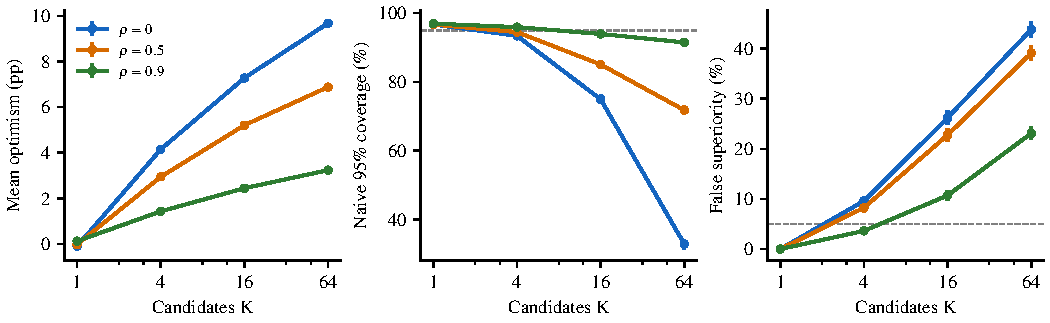
\includegraphics[width=\textwidth]{generated/synthetic.pdf}
\caption{Equal-accuracy Bernoulli candidates, $n=128$. Larger searches increase optimism, reduce ordinary interval coverage, and induce false paired superiority claims. Dependence attenuates all three effects. Error bars show 1.96 MCSE over 4,000 repetitions; dashed lines mark nominal coverage or error thresholds. The true gain is zero for every candidate.}
\label{fig:synthetic}
\end{figure*}

Figure~\ref{fig:synthetic} isolates selection from any genuine prompt improvement. With $n=128$, $K=64$, and independent correctness, mean optimism is \SynOptimism\ percentage points (pp), ordinary nominal 95\% coverage is \SynNaiveCover\%, and unadjusted paired testing falsely declares superiority in \SynNaiveFalseSuperiority\% of repetitions. In this construction every positive gain is spurious. These are experimentally observed failure rates, not values inferred from an asymptotic bound.

Increasing $\rho$ while holding marginal accuracy fixed reduces the optimism (Table~\ref{tab:synthetic}). The ordinary interval can appear satisfactory under strong dependence even though it lacks a general post-selection guarantee. Simultaneous exact intervals and independent audits retain at least nominal coverage in these settings; the former are conservative, especially when errors are strongly shared. The adjusted paired rule's false claim rate in the independent setting is \SynAdjustedFalseSuperiority\%, below its 5\% familywise upper bound. Appendix~\ref{app:full} reports the entire grid, including sample-size variation and the no-search control.

\begin{table*}[t]
\caption{Synthetic $K=64$, $n=128$: mean optimism in pp and coverage in percent, each $\pm1$ MCSE. The columns refer to ordinary reuse, simultaneous reuse, and an independent size-$n$ audit.}
\label{tab:synthetic}
\centering\small\begin{tabular}{lrrrr}
\toprule
$\rho$ & Optimism & Naive cov. & Simult. cov. & Audit cov. \\
\midrule
0.0 & 9.7 $\pm$ 0.03 & 32.9 $\pm$ 0.74 & 97.9 $\pm$ 0.23 & 96.8 $\pm$ 0.28 \\
0.5 & 6.9 $\pm$ 0.05 & 71.8 $\pm$ 0.71 & 98.5 $\pm$ 0.19 & 96.6 $\pm$ 0.29 \\
0.9 & 3.2 $\pm$ 0.06 & 91.5 $\pm$ 0.44 & 99.7 $\pm$ 0.09 & 97.0 $\pm$ 0.27 \\
\bottomrule
\end{tabular}

\end{table*}

\subsection{Real Prompts: Scores and Gains Have Different Meanings}
The real candidates' development accuracies range from \MinDev\% to \MaxDev\%. Pairwise correctness correlations average \MeanCorrelation\ (range \MinCorrelation--\MaxCorrelation), so neither independent arms nor identical arms describes this family. This is descriptive evidence from the development matrix, not an estimate of a universal effective number of prompts.

For a 24-candidate search on 128 replay questions, mean optimism is \RealOptimism\ pp. The reported gain over the fixed baseline is \RealReportedGain\ pp, while the actual gain on the empirical population is \RealActualGain\ pp. Equation~\eqref{eq:gains} explains their difference. Reuse can therefore distort the magnitude of a benefit without implying that the selected prompt has no benefit at all. Table~\ref{tab:real} and Figure~\ref{fig:real} show how the result changes with sample size; the $K=1$ control removes the selection step. The corresponding ordinary, simultaneous, and independent-audit coverages at $n=128$ are \RealNaiveCover\%, \RealSimultaneousCover\%, and \RealAuditCover\%.

\begin{figure}[t]
\centering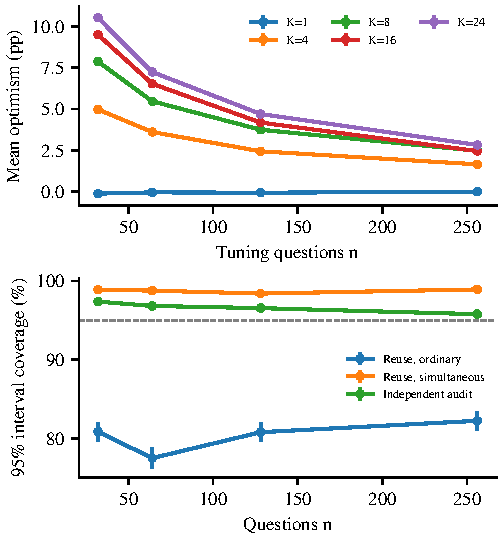
\includegraphics[width=\columnwidth]{generated/real_replay.pdf}
\caption{Real response matrix, empirical-population replay. Top: optimism depends on tuning size and the frozen nested candidate family. Bottom: interval coverage for $K=24$. Error bars are 1.96 MCSE and describe replay uncertainty conditional on the matrix.}
\label{fig:real}
\end{figure}

\begin{table*}[t]
\caption{Real-data replay with all 24 candidates: mean optimism (pp) and interval coverage (\%), $\pm1$ MCSE. The known target is the selected candidate's mean over the development population.}
\label{tab:real}
\centering\small\begin{tabular}{lrrrr}
\toprule
n & Optimism & Naive cov. & Simult. cov. & Audit cov. \\
\midrule
32 & 10.5 $\pm$ 0.08 & 80.8 $\pm$ 0.62 & 98.9 $\pm$ 0.16 & 97.4 $\pm$ 0.25 \\
64 & 7.2 $\pm$ 0.05 & 77.5 $\pm$ 0.66 & 98.8 $\pm$ 0.17 & 96.8 $\pm$ 0.28 \\
128 & 4.7 $\pm$ 0.04 & 80.8 $\pm$ 0.62 & 98.4 $\pm$ 0.20 & 96.5 $\pm$ 0.29 \\
256 & 2.8 $\pm$ 0.03 & 82.2 $\pm$ 0.60 & 98.9 $\pm$ 0.16 & 95.8 $\pm$ 0.32 \\
\bottomrule
\end{tabular}

\end{table*}

Across individual $n=128$, $K=24$ replay searches, the central 90\% of realized reuse errors lie between \RealOptimismQFive\ and \RealOptimismQNinetyFive\ pp, and \RealNegativeRate\% are negative. Expected optimism is therefore not a correction that identifies the error of one observed winning score. In the secondary heterogeneous simulation, a true 15-pp advantage yields an optimal-selection frequency of \HeteroLargeOptimal\% and mean optimism of \HeteroLargeOptimism\ pp; the appendix reports all gap settings. Mean separation attenuates the effect but does not automatically validate an ordinary interval.

\paragraph{The separate locked audit.}
The primary search selects candidate \PrimaryCandidate\ with a tuning score of \PrimaryTuneScore\%, versus \PrimaryBaselineTune\% for the fixed baseline. On 1,024 unused questions its score is \PrimaryAuditScore\%, with exact 95\% interval [\PrimaryLo, \PrimaryHi]\%; baseline accuracy is \PrimaryBaselineAudit\%. The selected-minus-baseline difference is \PrimaryAuditGain\ pp, with conservative exact 95\% paired-gain interval [\PrimaryGainLo, \PrimaryGainHi] pp. There are \PrimaryWins\ wins and \PrimaryLosses\ losses among paired discordances, giving one-sided paired $p=\PrimaryP$. The audit does not establish superiority at the 5\% level despite the positive tuning gain. This single locked comparison estimates the frozen configuration, not the expected result of rerunning optimization. It also cannot identify the exact population optimism: both the chosen and baseline audit accuracies remain estimates.

The additional audit-referenced mean optimism for the $n=128$, $K=24$ replay procedure is \RealAuditReferencedOptimism\ pp: mean reuse accuracy is \RealMeanReportedAccuracy\%, while selection-frequency-weighted accuracy on unused questions is \RealWeightedAuditAccuracy\%. The audit-only standard error of the difference is \RealAuditReferenceAuditSE\ pp; its MCSE is \RealAuditReferenceMCSE\ pp. This uses selection frequencies determined on development data and is conditional on that development population. It is an external check on the finite-pool analysis, not a known-truth coverage experiment.

\subsection{Reliable Reporting Has a Measurable Budget Cost}
\begin{figure*}[t]
\centering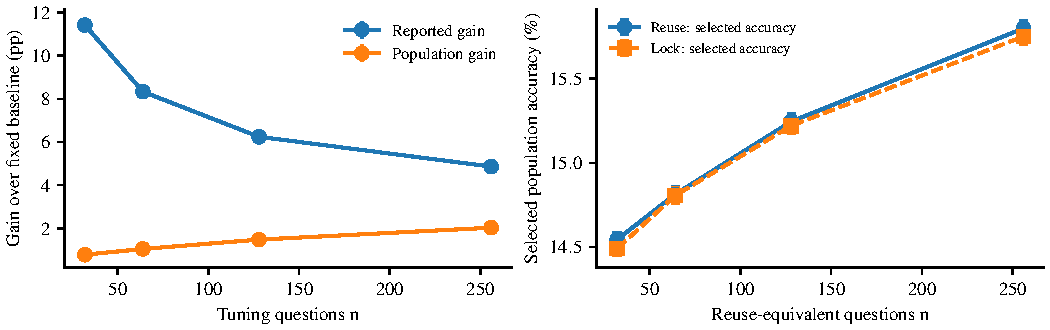
\includegraphics[width=\textwidth]{generated/gains_budget.pdf}
\caption{Real empirical-population replay. Left: reported versus actual gain over fixed candidate 0, using all 24 candidates. Right: quality of the selected configuration under reuse and the exactly matched call-budget audit allocation. Reliability and selection quality are separate outcomes. All error bars show 1.96 MCSE conditional on the empirical population.}
\label{fig:budget}
\end{figure*}

The call-budget comparison in Table~\ref{tab:budget} keeps $Kt+h=Kn$ exactly. The held-out protocol sacrifices $\lceil n/K\rceil$ tuning questions per candidate and spends those calls evaluating the winner on at least $n$ independent questions. Coverage, interval width, and the change in selected accuracy are all reported; a valid wide interval and a precisely selected configuration are different goals. Simultaneous intervals spend no additional calls but pay a multiplicity penalty in width. The locked-audit intervals avoid that penalty by requiring unused items. Figure~\ref{fig:budget} displays selection quality directly, rather than assuming that holding out data is costless.

\begin{table*}[t]
\caption{Exactly matched real-model call budgets, $K=24$. Coverage is percent; widths and selected-quality changes are pp. Coverage and quality differences include $\pm1$ MCSE. Simultaneous width is for the full reuse design; audit width is for the independent audit. $\Delta$ quality is audit-design selected accuracy minus reuse-design selected accuracy on the known empirical population, paired within each replay repetition.}
\label{tab:budget}
\centering\small\begin{tabular}{lrrrrr}
\toprule
Calls & Tune/audit & Audit cov. & Sim. width & Audit width & $\Delta$ quality \\
\midrule
768 & 30/48 & 96.5 $\pm$ 0.29 & 46.4 & 21.2 & -0.05 $\pm$ 0.02 \\
1536 & 61/72 & 96.5 $\pm$ 0.29 & 32.2 & 17.4 & -0.01 $\pm$ 0.02 \\
3072 & 122/144 & 96.3 $\pm$ 0.30 & 22.1 & 12.3 & -0.03 $\pm$ 0.02 \\
6144 & 245/264 & 95.8 $\pm$ 0.32 & 15.2 & 9.1 & -0.05 $\pm$ 0.01 \\
\bottomrule
\end{tabular}

\end{table*}

At 3,072 calls, tuning on 122 questions and auditing on 144 achieves \MatchedAuditCoverage\% coverage and mean width \MatchedAuditWidth\ pp, compared with \MatchedSimWidth\ pp for simultaneous reuse. The selected-quality change is \MatchedQualityDifference\ $\pm$ \MatchedQualitySE\ pp (one MCSE). These are conditional replay results, not a guarantee that the same allocation is optimal for other search families.

The equal-question split is a stricter limitation on available items: half the questions tune all configurations and half audit only the winner. Its full results appear in Appendix~\ref{app:full}. These two cost models should not be conflated. When fresh items are scarce rather than model calls, exact simultaneous reporting may be preferable despite wider intervals.

\paragraph{Duplicate-program stress test.}
We charge the same 24 programs either as 24 unique entries or as 192 entries formed by eight exact copies of each program. Selection scores and chosen population accuracies do not change; raw-count Bonferroni reporting widens. Appendix~\ref{app:duplicates} gives the measured widths and coverage. This deliberate representation change demonstrates a weakness of the conservative comparator, not a failure of its coverage guarantee. It also cautions against explaining selection noise using the number of logged trials without identifying which trials represent distinct functions.

\section{Discussion and Limitations}
\paragraph{What is supported.}
The experiments support three claims within the stated setting. Reusing a finite question set can inflate a selected score and cause incorrect comparison decisions. The size of this effect depends on sample size, means, and dependence, so no universal correction based solely on trial count is justified by these data. Finally, independent auditing and finite-family simultaneous inference restore validity under their explicit assumptions; the former has a favorable call-accounting structure when only one winning configuration must be deployed.

\paragraph{Where the guarantees stop.}
The simultaneous argument requires that all candidate functions be frozen independently of the evaluated questions. Counting only the configurations produced by a data-adaptive instruction generator does not supply a valid family size. As a boundary example, a program that memorizes observed gold labels and guesses elsewhere can score perfectly on its construction sample without transferring. A fresh locked audit still evaluates that final program honestly, provided it is not itself reused. Our real optimizer searches a predefined grid; it does not test adaptive proposal generation, multistage pipelines, or protected leaderboards.

\paragraph{Empirical limits.}
The real experiment has one small model, one benchmark, one quantization, and one decoding procedure. The prompt family combines instructions, punctuation, and option order; it is not representative of all automatic optimizers. Cached deterministic answers isolate selection from decoding noise. Fresh stochastic generations would add another source of variance and require a specified seed- or call-level target. Category clustering, duplicated questions, non-iid acquisition, or distribution shift can invalidate simple binomial population inference. Uniform iid draws from the development rows satisfy the replay assumptions by construction, but do not validate them for all natural questions.

The locked audit is unseen by the optimizer, not necessarily unseen during model pretraining. We cannot rule out benchmark contamination in the model. Its uncertainty is conditional on sampling questions from a relevant population and excludes uncertainty over different benchmark constructions. Observing many real candidate scores on an audit matrix does not license picking the best audit score after the fact. We retain all such scores for transparency and explicitly restrict the primary claim to the frozen choice.

\paragraph{Practical reporting recommendation.}
A report should identify the unit of search, the candidate-generation data, the number of distinct frozen configurations, the tuning questions, and the intended target. Report the reuse score as an optimization statistic. For a deployed winner, separately report an independent audit score and interval, a fixed paired baseline, and the consumed call and question budgets. If independent data are unavailable and the family truly was frozen, report a simultaneous interval together with its width and assumptions. To claim that an optimizer itself improves performance, repeat the entire selection process on independent outer splits and evaluate those selections on unused questions; an interval for one winner does not answer that question.

\section*{Impact Statement}
Overstated benchmark gains can misdirect deployment, purchasing, and research investment. Explicitly separating optimization scores from audited performance can improve accountability. Conversely, conservative intervals may hide useful improvements when evaluation resources are scarce, and an audited score can be misrepresented as a guarantee under distribution shift. Our release contains public benchmark text and locally generated answers, no private participant data, and does not make safety or general capability claims about the tested model.

\bibliography{references}
\bibliographystyle{icml2026}

\clearpage
\appendix
\onecolumn
\section{Proofs and Boundary Cases}\label{app:proofs}
\subsection{Nonnegativity and the Ordinary Bound}
Let $\mu_* =\max_j\mu_j$. Because $J$ is an empirical maximizer,
\begin{align*}
 O_n &=\E\max_j\muh_j-\E\mu_J\\
 &=\underbrace{\E\max_j\muh_j-\mu_*}_{\geq0\text{ by Jensen}}
   +\underbrace{\mu_*-\E\mu_J}_{\geq0}.
\end{align*}
This decomposition also distinguishes the upward bias of the empirical maximum as an estimate of the oracle accuracy from the regret of selecting a suboptimal candidate. For $X_j=\muh_j-\mu_j$, the selected error is bounded by $\max_jX_j$. The bounded Bernoulli moment generating function inequality gives $\E\exp(\lambda X_j)\leq\exp(\lambda^2/(8n))$. A log-sum-exp argument yields
\[
 \E\max_jX_j\leq\frac{\log K}{\lambda}+\frac{\lambda}{8n}.
\]
Optimizing over $\lambda>0$ gives Equation~\eqref{eq:hoeffding}. The same proof does not require independence between candidates. When $K=1$, the selected function is fixed and its empirical mean is unbiased.

\subsection{Contrast Variance Bound}
Set $D_j=Y_j-Y_0$ and $\delta_j=\E D_j$. Since $\E X_0=0$,
\[
 O_n=\E(X_J-X_0)\leq\E\max_j\{(\muh_j-\muh_0)-(\mu_j-\mu_0)\}.
\]
The centered contrast $D_j-\delta_j$ is bounded in absolute value by 2 and has variance at most $v$. Its sample-mean log moment generating function satisfies
\[
 \log\E\exp\{\lambda[(\muh_j-\muh_0)-(\mu_j-\mu_0)]\}
 \leq\frac{(v/n)\lambda^2}{2(1-2\lambda/(3n))},\qquad0<\lambda<3n/2.
\]
This follows by the usual exponential-series bound for a centered bounded random variable and iid row factorization. Applying log-sum-exp gives $\log K/\lambda+(v/n)\lambda/[2(1-2\lambda/(3n))]$. For $v>0$, take
\[
 \lambda=\frac{\sqrt{2\log K/(v/n)}}{1+(2/(3n))\sqrt{2\log K/(v/n)}}
\]
to obtain $\sqrt{2v\log K/n}+2\log K/(3n)$. If $v=0$, every contrast is constant almost surely and the actual expected optimism is zero. The displayed bound is still valid, though loose. When all programs are identical, the maximum contrast error vanishes exactly. The bound depends on a reference and is not a claim that a particular observed covariance estimate gives guaranteed post-selection inference.

\subsection{The Gaussian Calculation and Gains}
In Equation~\eqref{eq:gaussian}, the term containing $H$ is common to all candidates and does not affect the maximizing identity. The empirical maximum is that common term plus $\sigma\sqrt{1-\rho}\max_jG_j/\sqrt n$. The former has expectation zero, yielding Equation~\eqref{eq:gaussoptimism}. For iid standard normals, $\E\max_jG_j=\int_{-\infty}^{\infty}xK\phi(x)\Phi(x)^{K-1}dx$, an exact distributional expression; no numerical value from it is presented as experimental evidence. Taking expectations in Equation~\eqref{eq:gains} and using $\E(\muh_0-\mu_0)=0$ proves the gain identity. It fails for a baseline also selected using the same data without accounting for that selection.

\subsection{Exact Inference and the Paired Gain Interval}
The intervals in Equation~\eqref{eq:cp} invert equal-tailed binomial tests and hence have marginal coverage at least $1-\alpha$ for every success probability, including boundary probabilities. Applying the union bound to a frozen set of these intervals proves Equation~\eqref{eq:simultaneous}. For the independent audit, conditional coverage given all tuning data is at least $1-\alpha$; averaging over tuning preserves the guarantee. Neither proof assumes independent candidate responses.

Let $p_{10}$ and $p_{01}$ be probabilities of a candidate-only win and a baseline-only win on a new item. The difference in accuracies is $p_{10}-p_{01}$. Conditional on $W+L=d$, the number of wins has distribution $\operatorname{Bin}(d,p_{10}/(p_{10}+p_{01}))$ when $d>0$. Under the superiority null this probability is at most $1/2$, proving validity of the one-sided test. For $d=0$ set $p=1$. To give a conservative 95\% interval for the locked paired accuracy difference, separately compute binomial intervals $[L_W,U_W]$ and $[L_L,U_L]$ with failure probability $0.025$ each on the full audit size. The difference interval is $[L_W-U_L,U_W-L_L]$. A union bound proves its 95\% coverage without assuming that wins and losses are independent.

\section{Frozen Prompts, Data, and Computation}\label{app:implementation}
\paragraph{Instructions.}
Instruction 0 is: ``Answer the following multiple-choice question. Output only the letter of the correct option.'' Instruction 1 is: ``You are an expert in this subject. Carefully compare all options and choose the best answer. Output only its letter.'' Styles 0--2 render an option as \texttt{A. text}, \texttt{(A) text}, or \texttt{A: text}. Rotation $r\in\{0,1,2,3\}$ left-rotates the original options by $r$ before assigning display labels. The candidate ID is $12i+4f+r$, where $i$ is the instruction and $f$ is the style. The system message is ``You are a helpful assistant.'' The user message contains the instruction, question, options, and \texttt{Answer:}, in that order, using the model's ChatML delimiters. A grammar restricts the completion to one of the legal letters; exactly one token is generated greedily.

\paragraph{Versions and seeds.}
The pinned resources are:
\begin{itemize}
\item Dataset revision: \texttt{b189ec765aa7ed75c8acfea42df31fdae71f97be}.
\item Official model GGUF revision: \texttt{9217f5db79a29953eb74d5343926648285ec7e67}.
\item Model file: \texttt{qwen2.5-0.5b-instruct-q8\_0.gguf}.
\item llama.cpp commit: \texttt{785322d17f2d51e5185cf996a1f4e46d87640841}.
\end{itemize}
Question sampling and decoding use seed 20261102; synthetic sampling uses 77301 (primary) and 77302 (secondary); real replay uses 88302; the budget-correct paired-audit control uses 88303; candidate order uses 5539; the duplicate ablation uses 11003 and 22003. Ties are uniform by independent random priorities in replay and smallest-ID for the locked primary choice. Dependency versions are in \texttt{requirements-lock.txt}. Exact prompts and selected question IDs are in the release.

\paragraph{Measured computation.}
Inference runs on an Intel Xeon Gold 6230 CPU host. Although 40 logical cores are visible, the container quota is four CPU cores. There is no GPU and no external inference API is used. The retained real matrix contains \TotalResponses\ generated answer tokens and \EvaluatedTokens\ total evaluated prompt tokens including cached prefixes; \ComputedTokens\ prompt tokens are processed after prefix reuse. The wall-clock span between the first and last retained response is \InferenceHours\ hours, including the interrupted engineering pilots and pauses. The main inference server uses \ServerCpuHours\ CPU-hours and peaks at \PeakMemoryGiB\ GiB resident memory; these process statistics exclude the terminated first engineering server. Machine-readable run durations, CPU accounting, memory measurements, download and build attempts, and the full command line accompany the release. The initial proxy and oversubscription failures are documented in the reproduction notes.

\paragraph{Scope of repeated uncertainty.}
Real replay MCSEs use repeated iid draws from the same fixed development matrix. They estimate simulation error conditional on that matrix, not uncertainty over its original acquisition. For an additional audit-referenced score, let $\widehat\pi_j$ be the observed frequency of choosing configuration $j$ over replay draws. Its weighted audit response on item $i$ is $g_i=\sum_j\widehat\pi_jY_j(Z_i^{\rm audit})$. The reported audit-only standard error is the sample standard deviation of $g_i$ divided by $\sqrt{1024}$, conditional on development and the Monte Carlo frequencies. The MCSE of the replayed reported-minus-audit scores is stored separately. No interval derived from these conditional errors is advertised as uncertainty over completely fresh development datasets.

\section{Complete Experimental Grids}\label{app:full}
All entries in the following tables are generated from the supplied scripts and cached answers. Coverage and false-claim rates are percentages; optimism and width are percentage points. The complete CSVs additionally include one-MCSE values for every metric. ``False naive'' and ``False adj.'' count a significant selected paired comparison \emph{and} a nonpositive true gain, as a proportion of all repetitions. They are not conditional error rates among only the true-null selections.

\begin{table}[h]
\caption{All synthetic settings. Each row uses 4,000 repetitions. The true gain over the baseline is zero for every candidate.}
\centering\small\begin{tabular}{lrrrrrrrr}
\toprule
rho & n & k & Opt. & Naive & Simult. & Audit & False naive & False adj. \\
\midrule
0 & 32 & 1 & -0.1 & 96.7 & 96.7 & 96.6 & 0.0 & 0.0 \\
0 & 32 & 4 & 8.3 & 94.7 & 98.2 & 96.9 & 6.6 & 1.6 \\
0 & 32 & 16 & 14.5 & 80.9 & 99.2 & 96.5 & 19.4 & 1.1 \\
0 & 32 & 64 & 19.6 & 42.0 & 99.1 & 97.0 & 35.8 & 0.5 \\
0 & 128 & 1 & -0.1 & 96.7 & 96.7 & 97.1 & 0.0 & 0.0 \\
0 & 128 & 4 & 4.1 & 93.4 & 98.4 & 97.0 & 9.6 & 2.9 \\
0 & 128 & 16 & 7.3 & 74.9 & 98.5 & 96.9 & 26.2 & 2.2 \\
0 & 128 & 64 & 9.7 & 32.9 & 97.9 & 96.8 & 43.8 & 1.7 \\
0 & 512 & 1 & -0.0 & 95.9 & 95.9 & 95.7 & 0.0 & 0.0 \\
0 & 512 & 4 & 2.1 & 91.6 & 97.9 & 96.0 & 10.5 & 3.8 \\
0 & 512 & 16 & 3.6 & 70.2 & 98.1 & 95.3 & 27.1 & 2.2 \\
0 & 512 & 64 & 4.8 & 23.8 & 98.2 & 95.9 & 45.6 & 1.9 \\
0.5 & 32 & 1 & 0.0 & 96.5 & 96.5 & 96.5 & 0.0 & 0.0 \\
0.5 & 32 & 4 & 6.0 & 95.2 & 97.9 & 96.9 & 4.0 & 1.5 \\
0.5 & 32 & 16 & 10.4 & 88.2 & 99.4 & 96.9 & 13.2 & 0.5 \\
0.5 & 32 & 64 & 14.0 & 76.2 & 99.6 & 96.8 & 26.3 & 0.0 \\
0.5 & 128 & 1 & -0.0 & 96.7 & 96.7 & 96.8 & 0.0 & 0.0 \\
0.5 & 128 & 4 & 2.9 & 94.5 & 98.6 & 96.5 & 8.2 & 2.5 \\
0.5 & 128 & 16 & 5.2 & 85.0 & 98.7 & 96.6 & 22.8 & 2.1 \\
0.5 & 128 & 64 & 6.9 & 71.8 & 98.5 & 96.6 & 39.1 & 1.8 \\
0.5 & 512 & 1 & -0.0 & 96.3 & 96.3 & 95.6 & 0.0 & 0.0 \\
0.5 & 512 & 4 & 1.5 & 92.7 & 98.5 & 95.5 & 9.2 & 3.3 \\
0.5 & 512 & 16 & 2.6 & 82.6 & 98.4 & 95.3 & 25.9 & 2.9 \\
0.5 & 512 & 64 & 3.4 & 67.3 & 98.7 & 95.2 & 44.5 & 2.1 \\
0.9 & 32 & 1 & -0.1 & 96.6 & 96.6 & 97.0 & 0.0 & 0.0 \\
0.9 & 32 & 4 & 2.4 & 96.8 & 98.9 & 96.1 & 0.0 & 0.0 \\
0.9 & 32 & 16 & 4.3 & 95.5 & 99.7 & 96.9 & 0.2 & 0.0 \\
0.9 & 32 & 64 & 5.6 & 93.8 & 99.9 & 96.5 & 1.1 & 0.0 \\
0.9 & 128 & 1 & 0.1 & 96.9 & 96.9 & 96.4 & 0.0 & 0.0 \\
0.9 & 128 & 4 & 1.4 & 95.9 & 99.0 & 96.2 & 3.6 & 1.1 \\
0.9 & 128 & 16 & 2.4 & 93.9 & 99.2 & 96.5 & 10.7 & 0.1 \\
0.9 & 128 & 64 & 3.2 & 91.5 & 99.7 & 97.0 & 23.1 & 0.0 \\
0.9 & 512 & 1 & -0.0 & 96.0 & 96.0 & 95.5 & 0.0 & 0.0 \\
0.9 & 512 & 4 & 0.6 & 95.2 & 99.0 & 96.2 & 8.1 & 2.4 \\
0.9 & 512 & 16 & 1.1 & 93.0 & 99.6 & 95.7 & 21.5 & 1.9 \\
0.9 & 512 & 64 & 1.5 & 90.8 & 99.9 & 95.9 & 38.4 & 1.2 \\
\bottomrule
\end{tabular}

\end{table}
\clearpage
\begin{table}[h]
\caption{All real empirical-population replay settings. Each row uses 4,000 repetitions. The candidate order is fixed and nested, with candidate 0 always included.}
\centering\small\begin{tabular}{lrrrrrrr}
\toprule
n & k & Opt. & Naive & Simult. & Audit & False naive & False adj. \\
\midrule
32 & 1 & -0.1 & 98.5 & 98.5 & 97.7 & 0.0 & 0.0 \\
32 & 4 & 5.0 & 96.0 & 98.9 & 97.4 & 2.1 & 0.7 \\
32 & 8 & 7.9 & 90.8 & 98.8 & 97.8 & 2.4 & 0.2 \\
32 & 16 & 9.5 & 85.7 & 98.9 & 97.5 & 2.3 & 0.1 \\
32 & 24 & 10.5 & 80.8 & 98.9 & 97.4 & 3.3 & 0.2 \\
64 & 1 & -0.1 & 96.9 & 96.9 & 97.0 & 0.0 & 0.0 \\
64 & 4 & 3.6 & 93.8 & 98.5 & 96.7 & 3.6 & 0.9 \\
64 & 8 & 5.5 & 87.8 & 98.5 & 97.0 & 3.4 & 0.4 \\
64 & 16 & 6.5 & 81.8 & 98.8 & 96.8 & 3.0 & 0.2 \\
64 & 24 & 7.2 & 77.5 & 98.8 & 96.8 & 4.3 & 0.2 \\
128 & 1 & -0.1 & 97.1 & 97.1 & 97.0 & 0.0 & 0.0 \\
128 & 4 & 2.4 & 95.5 & 98.6 & 97.0 & 3.5 & 0.8 \\
128 & 8 & 3.7 & 88.4 & 98.6 & 96.3 & 3.3 & 0.6 \\
128 & 16 & 4.2 & 84.9 & 98.5 & 96.4 & 2.2 & 0.2 \\
128 & 24 & 4.7 & 80.8 & 98.4 & 96.5 & 3.6 & 0.2 \\
256 & 1 & -0.0 & 95.5 & 95.5 & 95.4 & 0.0 & 0.0 \\
256 & 4 & 1.6 & 93.3 & 98.6 & 95.5 & 2.9 & 0.8 \\
256 & 8 & 2.5 & 88.4 & 98.7 & 95.9 & 2.3 & 0.1 \\
256 & 16 & 2.4 & 86.0 & 99.0 & 96.0 & 1.4 & 0.1 \\
256 & 24 & 2.8 & 82.2 & 98.9 & 95.8 & 2.4 & 0.1 \\
\bottomrule
\end{tabular}

\end{table}

\begin{table}[h]
\caption{Equal-question comparison: half of a fixed total question budget tunes all candidates; half audits only the winner. The change in selected quality is relative to exhaustive reuse of all questions with $K=24$.}
\centering\small\begin{tabular}{lrrrr}
\toprule
Total n & Tune n & Audit coverage & Audit width & $\Delta$ quality \\
\midrule
32 & 16 & 98.2 $\pm$ 0.21 & 36.6 & -0.24 $\pm$ 0.02 \\
64 & 32 & 97.6 $\pm$ 0.24 & 26.1 & -0.29 $\pm$ 0.03 \\
128 & 64 & 96.6 $\pm$ 0.29 & 18.5 & -0.44 $\pm$ 0.03 \\
256 & 128 & 96.6 $\pm$ 0.29 & 13.0 & -0.58 $\pm$ 0.03 \\
\bottomrule
\end{tabular}

\end{table}

\section{Matched Budgets for Paired Superiority}
Auditing only the winner is sufficient for its accuracy, but comparing it to a baseline on unused items requires baseline answers too. This final-validation control, added after the primary analysis to correct the cost accounting, uses $Kt+2h=Kn$ with the allocation in Section 5.4 and a separate random seed. It does not change any primary draw. Both audit configurations are frozen before their shared audit items are drawn. An audit with a baseline identical to the winner cannot claim superiority; the budget reserves both call streams conservatively. ``False claims'' counts a significant paired test with nonpositive true empirical-population gain, among all repetitions. The ordinary reuse comparison uses its unadjusted selected paired test with the same total call budget. Baseline and winner audits are both charged in the table below.
\begin{table}[h]
\caption{Paired decisions at exactly matched model-call budgets, $K=24$, 4,000 repetitions. The audit count is per configuration, so the audit costs twice that number of calls. False-claim frequencies and selected accuracy are percent $\pm1$ MCSE. Mixed true and null candidates mean these unconditional frequencies are not conditional type-I errors among only null selections.}
\centering\small\begin{tabular}{lrrrrr}
\toprule
Calls & Tune n & Audit n each & Reuse false claims & Audit false claims & Selected accuracy \\
\midrule
768 & 29 & 36 & 3.3 $\pm$ 0.28 & 0.5 $\pm$ 0.11 & 14.5 $\pm$ 0.02 \\
1536 & 58 & 72 & 4.3 $\pm$ 0.32 & 0.4 $\pm$ 0.11 & 14.8 $\pm$ 0.02 \\
3072 & 117 & 132 & 3.6 $\pm$ 0.29 & 0.3 $\pm$ 0.09 & 15.1 $\pm$ 0.02 \\
6144 & 234 & 264 & 2.4 $\pm$ 0.24 & 0.2 $\pm$ 0.07 & 15.7 $\pm$ 0.02 \\
\bottomrule
\end{tabular}

\end{table}

\section{Heterogeneous-Mean Secondary Control}
At fixed search size and sample size, this control varies only the true advantage of a single candidate over the other candidates. At zero gap every candidate is optimal, so the optimal-selection probability is one by definition. For positive gaps only the strengthened candidate is optimal. The experiment isolates mean separation from changes in candidate count or covariance; all settings use independent Bernoulli correctness across candidates before selection.
\begin{table}[h]
\caption{Secondary heterogeneous means, $K=64$, $n=128$, 4,000 repetitions. True gap, optimism, and oracle regret are pp; probabilities and coverage are percent. Entries are mean $\pm1$ MCSE.}
\centering\small\begin{tabular}{lrrrrr}
\toprule
True gap & P(optimal) (\%) & Optimism & Oracle regret & Naive cov. & Audit cov. \\
\midrule
0.0 & 100.0 $\pm$ 0.00 & 9.7 $\pm$ 0.03 & 0.0 $\pm$ 0.00 & 31.6 $\pm$ 0.74 & 96.8 $\pm$ 0.28 \\
2.0 & 4.1 $\pm$ 0.31 & 9.7 $\pm$ 0.03 & 1.9 $\pm$ 0.01 & 31.5 $\pm$ 0.73 & 96.5 $\pm$ 0.29 \\
5.0 & 15.7 $\pm$ 0.57 & 9.3 $\pm$ 0.04 & 4.2 $\pm$ 0.03 & 36.7 $\pm$ 0.76 & 96.2 $\pm$ 0.30 \\
15.0 & 86.7 $\pm$ 0.54 & 2.3 $\pm$ 0.08 & 2.0 $\pm$ 0.08 & 87.1 $\pm$ 0.53 & 95.8 $\pm$ 0.32 \\
\bottomrule
\end{tabular}

\end{table}

\section{Program-Duplication Ablation}\label{app:duplicates}
The response matrix and exhaustive selection are identical in both rows below. The only difference is whether the simultaneous interval uses $K=24$ or $K=192$, corresponding to counting eight exact copies of each program. Both satisfy a union-bound guarantee, but raw accounting overpays for entries that are known to be the same function. This exercise uses known program identity; it does not support data-dependent deduplication based on coincident answers.
\begin{table}[h]
\caption{Duplicate-program ablation, real empirical population, $n=128$. Entries are mean $\pm1$ MCSE; optimism and width are pp, coverage is percent.}
\centering\small\begin{tabular}{lrrr}
\toprule
Charged K & Optimism & Coverage & Width \\
\midrule
24 & 4.8 $\pm$ 0.04 & 98.6 $\pm$ 0.18 & 22.1 $\pm$ 0.01 \\
192 & 4.8 $\pm$ 0.04 & 99.8 $\pm$ 0.07 & 26.0 $\pm$ 0.02 \\
\bottomrule
\end{tabular}

\end{table}

\clearpage
\section{All Real Configurations}
\begin{table}[h]
\caption{Descriptive accuracies of all frozen configurations. These audit scores are released for transparency; they are not used to replace the locked primary choice. Each split contains 1,024 questions.}
\centering\small\begin{tabular}{lrrrrr}
\toprule
ID & Instruction & Style & Rotation & Dev. (\%) & Audit (\%) \\
\midrule
0 & 0 & 0 & 0 & 13.8 & 14.0 \\
1 & 0 & 0 & 1 & 14.9 & 15.5 \\
2 & 0 & 0 & 2 & 14.1 & 14.8 \\
3 & 0 & 0 & 3 & 17.4 & 14.6 \\
4 & 0 & 1 & 0 & 13.2 & 14.2 \\
5 & 0 & 1 & 1 & 13.5 & 15.0 \\
6 & 0 & 1 & 2 & 12.4 & 13.5 \\
7 & 0 & 1 & 3 & 15.1 & 13.9 \\
8 & 0 & 2 & 0 & 15.1 & 13.1 \\
9 & 0 & 2 & 1 & 13.3 & 15.2 \\
10 & 0 & 2 & 2 & 13.4 & 13.9 \\
11 & 0 & 2 & 3 & 14.8 & 15.4 \\
12 & 1 & 0 & 0 & 13.2 & 13.3 \\
13 & 1 & 0 & 1 & 14.6 & 14.0 \\
14 & 1 & 0 & 2 & 12.3 & 13.4 \\
15 & 1 & 0 & 3 & 14.2 & 12.8 \\
16 & 1 & 1 & 0 & 13.9 & 13.2 \\
17 & 1 & 1 & 1 & 15.2 & 14.2 \\
18 & 1 & 1 & 2 & 11.8 & 13.8 \\
19 & 1 & 1 & 3 & 13.7 & 12.9 \\
20 & 1 & 2 & 0 & 12.9 & 13.1 \\
21 & 1 & 2 & 1 & 14.1 & 14.5 \\
22 & 1 & 2 & 2 & 12.5 & 13.7 \\
23 & 1 & 2 & 3 & 14.3 & 13.2 \\
\bottomrule
\end{tabular}

\end{table}

\section{Completed Reproducibility and Ethics Checklist}
ICML 2026 requires an impact statement, provided before the references, and does not supply a mandatory in-paper NeurIPS-style questionnaire in the official template or author instructions consulted. We additionally complete the following study-specific checklist.
\begin{enumerate}
\item \textbf{Are the primary claims and their scope specified? Yes.} Sections 3--5 distinguish selected accuracy, optimizer value, and gain. Section 7 limits the claims to fixed-family selection, stated sampling distributions, and a small constrained-decoding model.
\item \textbf{Are assumptions and proofs supplied? Yes.} Independent question sampling, fixed candidate functions for simultaneous inference, and independent audit data are stated. Appendix~\ref{app:proofs} proves the bounds, coverage statements, paired test, and paired-gain interval.
\item \textbf{Is there real-model evidence from newly generated answers? Yes.} The release caches all \TotalResponses\ locally generated model answers, with hashes, settings, and correctness. No supplied or externally cached benchmark predictions are used.
\item \textbf{Are uncertainty and repeated runs described accurately? Yes.} Repeated synthetic experiments and conditional real replay have 4,000 repetitions each. MCSEs, ordinary and simultaneous coverage, and the single locked-audit interval are distinguished. We do not present replay as independent replications of benchmark acquisition.
\item \textbf{Are data, model, code, seeds, and dependencies available? Yes.} The reproduction package contains pinned download commands, the exact sampled items and configurations, raw outputs, statistical scripts, dependency lock file, seeds, and commands for every figure and table. Model weights are downloadable rather than embedded in the compact archive.
\item \textbf{Is compute and failure reporting provided? Yes.} Appendix~\ref{app:implementation} gives measured inference quantities. The logs record initialization failures, the CPU-quota correction, protocol amendments, and durations. No failed or uncompleted setting is silently counted as a successful experiment.
\item \textbf{Was a locked audit protected from optimizer feedback? Yes.} The primary winner is saved before any audit response is generated, and the analysis verifies this integrity record. Other audit scores are descriptive only.
\item \textbf{Are baselines and ablations appropriate? Yes, within scope.} No-search, ordinary exact intervals, paired tests, simultaneous exact intervals, independent audits, controlled correlation, question and call budgets, and program duplication are evaluated. Adaptive prompt generators, larger models, multistage systems, and distribution shifts are not evaluated.
\item \textbf{Are limitations and potential negative impacts discussed? Yes.} Section 7 and the impact statement discuss finite-pool targets, contamination, non-iid items, misuse under shift, scarce audit data, and conservative reporting.
\item \textbf{Are licenses and participant issues addressed? Yes.} Dataset/model cards and software licenses are recorded in the reproduction notes. The study uses public benchmark items with no recruited participants, private data, or human annotation. No participant compensation applies.
\item \textbf{Is AI assistance disclosed? Yes.} An autonomous language-model coding agent designed and implemented the analysis, accessed the permitted sources, and drafted the paper. The empirical answers come from the separately run, identified Qwen model. All numerical claims are generated from executable results, not from the drafting agent's unsupported predictions.
\item \textbf{Was the prohibited research material avoided? Yes, to the extent known.} Only the supplied starter papers and direct official data, model, infrastructure, and conference sources were accessed. No search for the unidentified excluded paper was performed. The source-access record reports any accidental exposure; none was knowingly encountered.
\end{enumerate}
\end{document}
